\section{Introduction}

\begin{frame}
\frametitle{Our tasks}
  \begin{itemize}
  \item Implement five different skjghkjgkjggets

	\begin{itemize}
		\item Reference Set using a C++11 std::set
        \item Fine grained locking Set
        \item Optimistic synchronization Set
        \item Lazy synchronization Set
        \item Lockfree Set
	\end{itemize}
   
  \item find/implement a benchmarking process
  \item evaluate the set performance
  \end{itemize}
\end{frame}

%------------------------------------------------
\section{More detailed set description}

\begin{frame}[fragile] % Need to use the fragile option when verbatim is used in the slide
\frametitle{Set Interface}
\begin{lstlisting}
class AMPSet {
[...]
	//adds an item to the set [...]
	virtual bool add(long item) = 0;
	
	//removes an item from the set [...]
	virtual bool remove(long item) = 0;
	
	//checks if an item is contained in a set [...]
	virtual bool contains(long item) = 0;
};
\end{lstlisting}
\end{frame}

\begin{frame}
\frametitle{Reference}
\begin{itemize}
	\item Used C++11 \texttt{std::set}
    \item synchronized each call to the object with a global \texttt{std::mutex}
    \item lock, since it is not thread safe
\end{itemize}

Basic information
\begin{itemize}
	\item \texttt{std::set} is based on a binary search tree
    \item our implementations will be based on simple lists
    \item the difference is going to be interesting
\end{itemize}
\end{frame}

\begin{frame}
\frametitle{Fine grained locking}
\begin{itemize}
	\item *no* global lock, but individual node locking
    \item \(\Rightarrow\) multiple threads can operate at the same time on different locations of the list
    \item deadlock free, because of the lock ordering
    \item linearization point if item in set is at the corresponding locking, otherwise at the parents node locking
\end{itemize}
\end{frame}

\begin{frame}
\frametitle{Optimistic synchronization}
\begin{itemize}
	\item does not lock any nodes during search, but when its found
    \item locked are the found element and its predecessor
    \item Requires validation that the nodes are still in list
    \begin{itemize}
		\item Q: What happens if that's not the case? 
        \item restart necessary 
	\end{itemize}
\end{itemize}
\end{frame}

\begin{frame}
\frametitle{Lazy synchronization}
\begin{itemize}
	\item does not acquire locks for \texttt{contains} checks
    \item ability to flag a node as \textit{removed}
    \item consequence: locally removed, but may still be linked
\end{itemize}
\end{frame}

\begin{frame}
\frametitle{Lockfree}
\begin{itemize}
	\item no locks at all, but \textit{hardware} atomic operations
    \item hardware support is provided due to combining pointer and flag into an atomic unit
    \item AMD64 .. 48bit with 64bit alignment
    \item SPARC T5 .. Physical 48bit (T4 44bit)
    \item tricky to implement
\end{itemize}
\end{frame}

%------------------------------------------------
\section{Everything else we did}

\subsection{Timer Benchmarking}
\begin{frame}[fragile]
\frametitle{Timer benchmark}
Benchmarking the timer, we ran each time measurement 1000 times

\begin{lstlisting}
// c++11 steady clock - <chrono>
std::chrono::steady_clock::now();

// c++11 high res clock - <chrono>
std::chrono::high_resolution_clock::now();

// monotonic clock - <include/time.h>
clock_gettime(CLOCK_MONOTONIC, &tmpTimeNow);

// get time of day - <sys/time.h>
gettimeofday(&start, NULL);

// system clock - <include/time.h>
clock();
\end{lstlisting}
\end{frame}

\begin{frame}
C++11 and Linux timer benchmarking, 649 datasets
\begin{figure}[H]
  \centering 
  \includegraphics[height=0.90\textheight]{pictures/timer_benchmarks.eps}
\end{figure}
\end{frame}

\subsection{Debugging of the LFS}

% Need to use the fragile option when verbatim is used in the slide
\begin{frame}[fragile]
\frametitle{We found bugs in the way of locking of the LFS}

Node unlinked after mark
\begin{lstlisting}
if(isMarked(w.curr)) {
    next = mark(next);
}
__sync_bool_compare_and_swap(
        &(getPointer(w.pred)->next), 
        w.curr, next);
\end{lstlisting}
\end{frame}

\begin{frame}[fragile]
Node was removed just after 'find' found it unmarked
\begin{lstlisting}
bool LockFreeSet::add(long item) {
  LfsNode *n = new LfsNode(item, nullptr);
  while (true) {
    LfsWindow w = find(item);	
    if(isMarked(w.curr)) {
      continue;
    }
  [...]
  }
}
\end{lstlisting}
\end{frame}


%------------------------------------------------
\section{Evaluation}

\begin{frame}
\frametitle{what did we analyze?}
You are able to do a lot of benchmarks, a lot lot. We did the following:
\begin{itemize}
	\item Performance comparison, with respect to throughput
    \begin{itemize}
		\item between two machines [mars, ceres]
        \item between four sets [REF, OS, LS, LF] (why *not* FGL)
        \item between four operation types [insert, contains, remove, mixed]
	\end{itemize}
    \item thread fairness comparison
    \begin{itemize}
    	\item between two machines [mars, ceres]
		\item between five sets [REF, FGL, OS, LS, LF]
        \item with just one operation type (why one)
	\end{itemize}
\end{itemize}
\end{frame}

\begin{frame}
\frametitle{Expectations}
\begin{itemize}
	\item a much faster reference set in single threaded mode
    \item at the beginning unknown expectations concerning parallel behavior 
\end{itemize}
\end{frame}

\subsection{Throughput}
\begin{frame}
\begin{figure}[H]
  \centering
\begin{tabular}{ l | c c c c }
 & add & contains & remove & mixed\\
 \hline
reference & 418.53 &  231.50 &  470.04  & 272.85\\
optimistic sync. & 2609.88  & 418.71 & 3421.86 &   38.19\\
lazy sync. & 1333.05 &  289.80 &  215.82  &  25.22\\
lock free & 1128.28  & 161.50  & 115.61   & 29.39\\
\end{tabular}
%  \caption{Average time in milliseconds of 100 throughput benchmark runs on Mars, 80 threads, 1000 iterations per thread}
\end{figure}
Average time in milliseconds of 100 throughput benchmark runs on Mars, 80 threads, 1000 iterations per thread

\begin{figure}[H]
  \centering
\begin{tabular}{ l | c c c c }
 & add & contains & remove & mixed\\
 \hline
reference & 29.75  &  25.17  &  25.77 &   27.94 \\
optimistic sync. & 1348.86 &  634.34 & 2344.10  &  39.79 \\
lazy sync. & 635.12  & 328.49 &  307.21  &  30.92 \\
lock free & 687.51  & 320.21 &  358.25  &  16.03\\
\end{tabular}
%  \caption{Average time in milliseconds of 100 throughput benchmark runs on Ceres, 64 threads, 1000 iterations per thread}
\end{figure}
Average time in milliseconds of 100 throughput benchmark runs on Ceres, 64 threads, 1000 iterations per thread
\end{frame}

\subsection{Fairness}
\begin{figure}[H]
  \centering 
  \includegraphics[height=0.90\textheight]{pictures/mars_fairness_plot.eps}
  %\caption{Histograms of 5 second runs on Mars with 80 threads}
  \label{marsfairness}
\end{figure}
Histograms of 5 second runs on Mars with 80 threads


\begin{figure}[H]
  \centering
  \includegraphics[height=0.90\textheight]{pictures/ceres_fairness_plot.eps}
  %\caption{Histograms of 5 second runs on Ceres with 500 threads}
  \label{ceresfairness}
\end{figure}
Histograms of 5 second runs on Ceres with 500 threads


%------------------------------------------------
\begin{frame}
\Huge{\centerline{Thank you}}
\end{frame}
%------------------------------------------------
